\section{Experiments}
\label{sec:experiments}
\begin{table*}[tb]
    \centering
    \small
    \begin{tabular}{l|r@{\ \ }rr@{\ \ }rr@{\ \ }r|r@{\ \ }rr@{\ \ }rr@{\ \ }r}
    \toprule
        & \multicolumn{6}{c|}{Character Error Rate} &\multicolumn{6}{c}{Word Error Rate} \\
        & \multicolumn{2}{c}{Ainu} & \multicolumn{2}{c}{Griko} & \multicolumn{2}{c|}{Yakkha} & \multicolumn{2}{c}{Ainu} & \multicolumn{2}{c}{Griko} & \multicolumn{2}{c}{Yakkha} \\[-0.3em]
        Model & \small Multi & \small Single & \small Multi & \small Single & \small Multi & \small Single & \small Multi & \small Single & \small Multi & \small Single & \small Multi & \small Single\\
        \midrule
        \textsc{Fp-Ocr} & \multicolumn{1}{c}{--} & $1.34$ & \multicolumn{1}{c}{--} & $3.27$ & \multicolumn{1}{c}{--} & $8.90$ & \multicolumn{1}{c}{--} & $6.27$ & \multicolumn{1}{c}{--} & $15.63$ & \multicolumn{1}{c}{--} & $31.64$ \\
        \textsc{Base} & $1.56$ & $1.41$ & $6.78$ & $5.95$ & $70.39$ & $71.71$ & $8.56$ & $7.88$ & $15.13$ & $13.67$ & $98.15$ & $99.10$  \\
        \textsc{Copy} & $2.04$ & $1.99$ & $2.54$ & $2.28$ & $14.77$ & $12.30$ & $9.48$ & $8.57$ & $9.33$ & $8.90$ & $30.36$ & $27.81$ \\
        \textsc{Ours} & $0.92$ & $\boldsymbol{0.80}$ & $\boldsymbol{1.66}$ & $1.70$ & $\boldsymbol{7.75}$ & $8.44$ & $5.75$ & $\boldsymbol{5.19}$ & $\boldsymbol{7.46}$ & $7.51$ & $\boldsymbol{20.95}$ & $21.33$ \\
    \bottomrule
    \end{tabular}
    \caption{Our method improves performance over all baselines (10-fold cross-validation averaged over five randomly seeded runs). We present multi- and single-source variants and \textbf{highlight} the best model for each language.}
    \label{tab:cer}
\end{table*}

This section discusses our experimental setup and the post-correction performance on the three endangered languages on our dataset.

\subsection{Experimental Setup}
\smallskip
\paragraph{Data Splits}
We perform 10-fold cross-validation for all experimental settings because of the small size of the datasets. For each language, we divide the transcribed data into 11 segments --- we use one segment for creating the \emph{denoising rules} described in the previous section and the remaining ten as the folds for cross-validation. In each cross-validation fold, eight segments are used for training, one for validation and one for testing.

We divide the dataset at the page-level for the Ainu and Griko documents, resulting in 11 segments of three pages each. For the Yakkha documents, we divide at the paragraph-level, due to the small size of the dataset. We have 33 paragraphs across the three books in our dataset, resulting in 11 segments that contain three paragraphs each. The multi-source results for Yakkha reported in \autoref{tab:cer} use the English translations. Results with Nepali are similar and are included in \autoref{sec:appendix}.

\paragraph{Metrics}
We use two metrics for evaluating our systems: character error rate (CER) and word error rate (WER). Both metrics are based on edit distance and are standard for evaluating OCR and OCR post-correction~\cite{berg-kirkpatrick-etal-2013-unsupervised,schulz-kuhn-2017-multi}. 
CER is the edit distance between the predicted and the gold transcriptions of the document, divided by the total number of characters in the gold transcription. WER is similar but is calculated at the word level.

\paragraph{Methods}
In our experiments, we compare the performance of our proposed method with the first pass OCR and with two systems from recent work in OCR post-correction. All the post-correction methods have two variants -- the single-source model with only the endangered language encoder and the multi-source model that additionally uses the high-resource translation encoder.
\begin{itemize}
    \item \textsc{Fp-Ocr}: The first pass transcription obtained from the Google Vision OCR system.
    \item \textsc{Base}: This system is the base sequence-to-sequence architecture described in \autoref{sec:base}. Both the single-source and multi-source variants of this system are used for English OCR post-correction in~\citet{dong-smith-2018-multi}. 
    \item \textsc{Copy}: This system is the base architecture with a copy mechanism as described in \autoref{sec:recipe1}. The single-source variant of this model is used for OCR post-correction on Romanized Sanskrit in \citet{krishna-etal-2018-upcycle}.\footnote{Although~\citet{krishna-etal-2018-upcycle} use BPE tokenization, preliminary experiments showed that character-level models result in much better performance on our dataset, likely due to the limited data available for training the BPE model.}
    \item \textsc{Ours}: The model with all the adaptations proposed in \autoref{sec:recipe1} and \autoref{sec:recipe2}.
\end{itemize}

\paragraph{Implementation} The post-correction models are implemented using the DyNet neural network toolkit~\cite{dynet}, and all reported results are the average of five training runs with different random seeds. We assume knowledge of the entire alphabet of the endangered language for all the methods, which is straightforward to obtain for most languages. The decoder's vocabulary contains all these characters, irrespective of their presence in the training data, with corresponding randomly-initialized character embeddings.

\subsection{Main Results}
\label{sec:results}
\renewcommand{\arraystretch}{1.0}
\begin{figure*}[tb]
    \centering
    \small
    \begin{tabular}{lcc}
    & \multicolumn{2}{c}{Errors \textit{fixed} by post-correction}\\[.1cm]
        & (a) Griko & (b) Yakkha  \\
        \raisebox{0.7em}{[Image]} & \frame{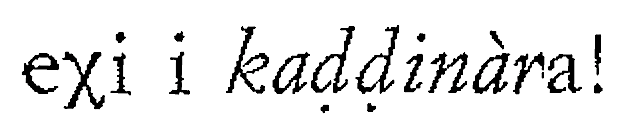
\includegraphics[width=0.4\columnwidth]{images/errors1a.pdf}} & \frame{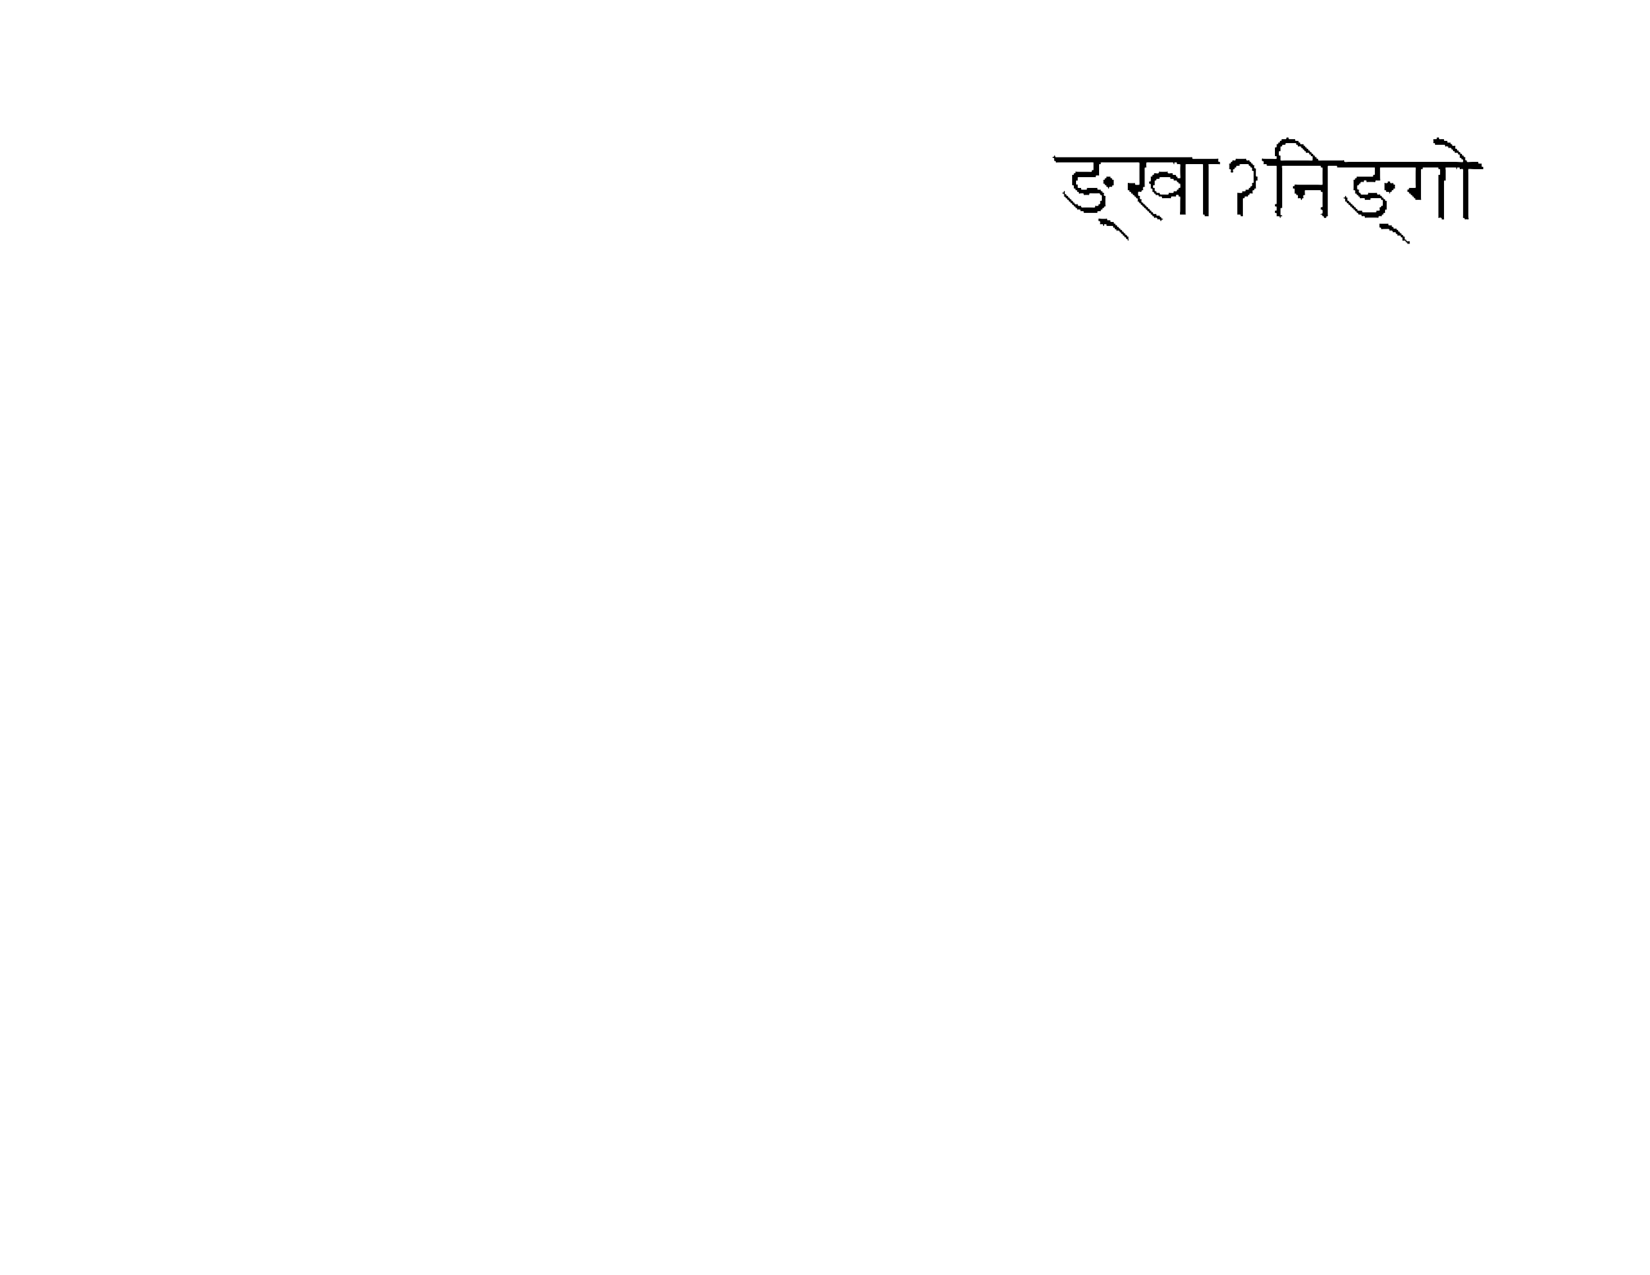
\includegraphics[width=0.3\columnwidth]{images/errors2a.pdf}} \\
        & \multicolumn{2}{c}{$\big\downarrow$ \hspace{3cm} $\big\downarrow$}\\
        \raisebox{0.35em}{[First pass OCR]} & \raisebox{0.3em}{\large e\textcolor{burntred}{\textbf{x}}i i ka\textcolor{burntred}{\textbf{dd}}in\`ara} &
        
\includegraphics[width=0.25\columnwidth]{images/error2b.pdf} \\
        & \multicolumn{2}{c}{$\big\downarrow$ \hspace{3cm} $\big\downarrow$}\\
        \raisebox{0.35em}{[Post-corrected]} & \raisebox{0.35em}{\large e\textcolor{burntblue}{$\bm{\chi}$}i i ka\textbf{\textcolor{burntblue}{\d{d}\d{d}}}in\`ara} &
        
\includegraphics[width=0.28\columnwidth]{images/error2c.pdf} \\
    \end{tabular}
    \qquad
    \begin{tabular}{cc}
        \multicolumn{2}{c}{Errors \textit{introduced} by post-correction}\\[.1cm]
        (c) Griko & (d) Yakkha  \\
        \frame{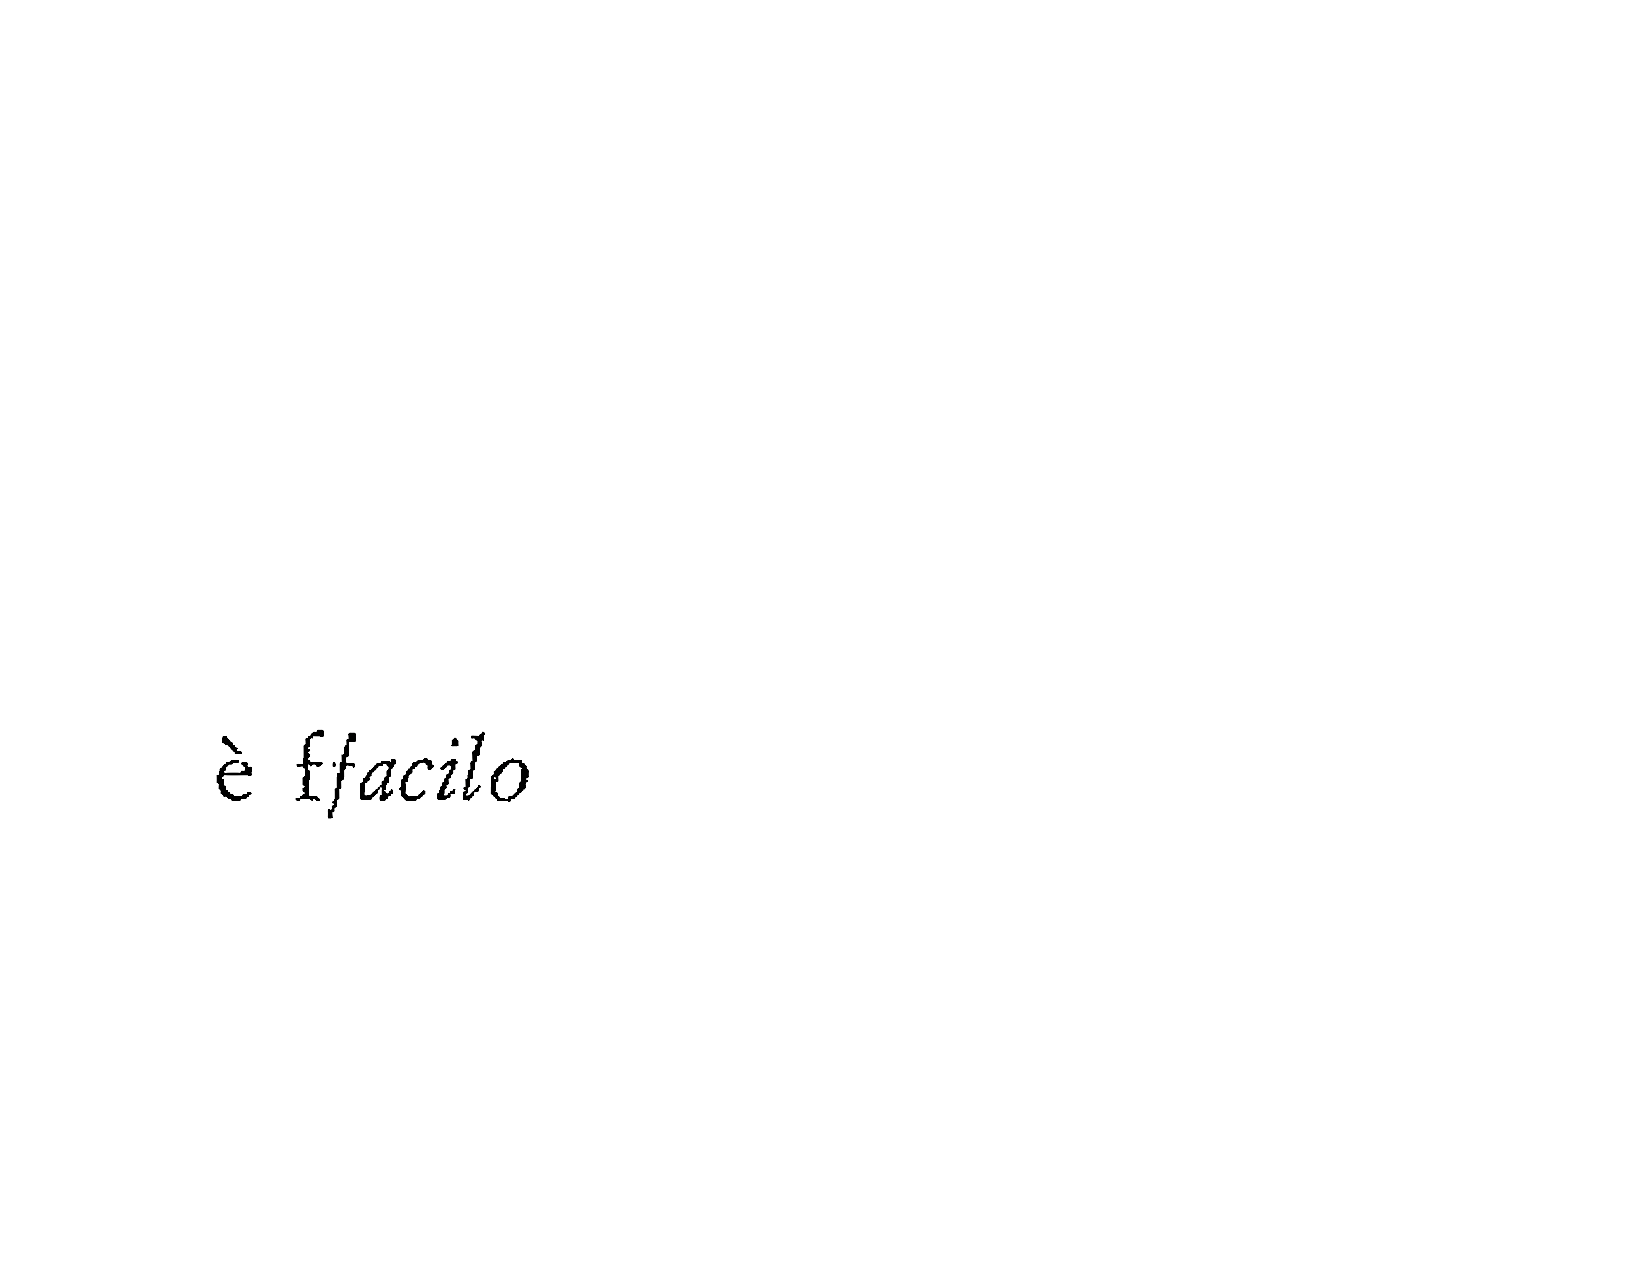
\includegraphics[width=0.25\columnwidth]{images/errors3a.pdf}} & \frame{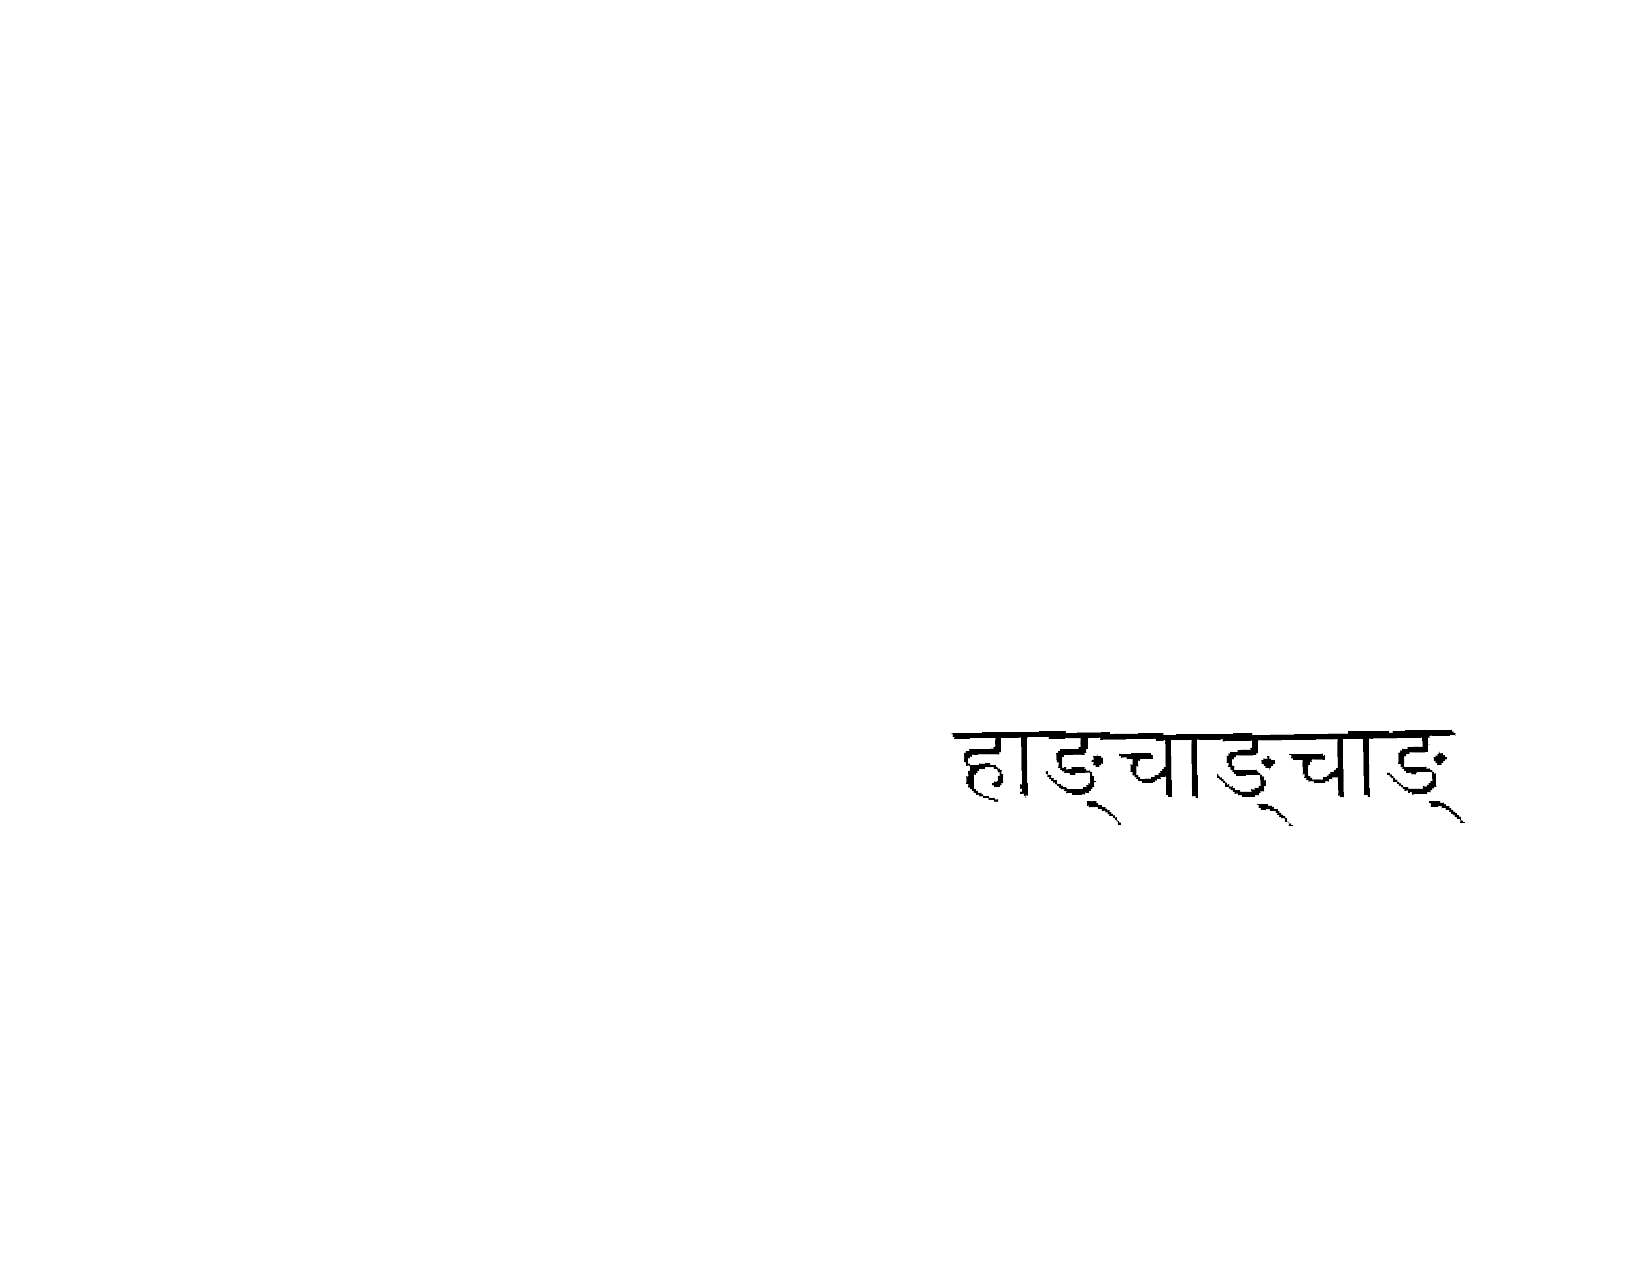
\includegraphics[width=0.35\columnwidth]{images/errors4a.pdf}} \\
        \multicolumn{2}{c}{$\big\downarrow$ \hspace{2.5cm} $\big\downarrow$}\\
        \raisebox{0.35 em}{\large{\`{e} ffacilo}} &
        
\includegraphics[width=0.3\columnwidth]{images/errors4b.pdf} \\
        \multicolumn{2}{c}{$\big\downarrow$ \hspace{2.5cm} $\big\downarrow$}\\
        \raisebox{0.35 em}{\large{\`{e} ffa\textcolor{burntred}{\textbf{\'{c}}}ilo}} &
        
\includegraphics[width=0.32\columnwidth]{images/errors4c.pdf}
    \end{tabular}
    \caption{Our model fixes many mixed script and uncommon diacritics errors such as (a) and (b). In rare cases, it ``over-corrects" the first pass OCR transcription, introducing errors such as (c) and (d).}
    \label{fig:error_examples}
\end{figure*}

\begin{figure}[t]
    \definecolor{graphblue}{HTML}{A6BDDB}
\pgfplotstableread[row sep=\\,col sep=&]{
det & Ainu & Griko & Yakkha \\
all & 5.19 & 7.46 & 24.29 \\
diag & 5.49 & 8.06 & 22.73 \\
copy & 6.56 & 8.66 & 37.83 \\
coverage & 5.60 & 10.19 & 26.71 \\
dec & 6.86 & 7.87 & 20.95 \\
enc & 6.70 & 9.47 & 28.41 \\
seq2seq & 5.65 & 9.43 & 27.68 \\
}\data
\def\mystrut{\vphantom{hp}}

%\vspace{-1em}
\begin{tikzpicture}[trim left=-1.6cm,trim right=0cm]
    \begin{axis}[
            xbar,
            every axis plot post/.style={/pgf/number format/fixed},
            bar width=.23cm,
            width=4cm,
            height=4cm,
            ymajorgrids=false,
            yminorgrids=false,
            xmajorgrids=false,
            %every axis legend/.code={\let\addlegendentry\relax},
            %legend={Wikipedia Size (in million articles)},
            legend style={draw=none,at={(0.2,0.9)},anchor=west},
            symbolic y coords={all,diag,copy,coverage,dec,enc,seq2seq},
            ytick={all,diag,copy,coverage,dec,enc,seq2seq},
            yticklabels={all,-diag,-copy,-coverage,-pretr. dec,-pretr. enc,-pretr. s2s},
            %ytick={all,-diag loss,-copy,-coverage, -pretrain dec,-pretrain enc,-pretrain seq2seq},
            every y tick label/.append style={font=\small\mystrut},
            every x tick label/.append style={font=\small\mystrut},
            tick pos=left,
            %hide y axis,
            axis x line*=bottom,
            axis y line*=left,
            nodes near coords,
            %nodes near coords align={vertical},
            every node near coord/.append style={font=\small,color=black},
            %nodes near coords style={},
            title={\small Ainu},
            title style={yshift=-0.3cm},
            %ymin=0,ymax=6.1,
            xmin=0,xmax=8,
            %ylabel shift={-1cm},
            %ylabel near ticks,
            %ylabel={},
            %xlabel near ticks,
            %xlabel={WER},
            enlarge x limits=0.0,
            xtick style={draw=none}
        ]
        %\addplot [style={black,postaction={pattern=north east lines},fill=white,mark=none}] table[x=story,y=base]{\ainudata};
        \addplot [style={graphblue,fill=graphblue,mark=none}] table[x=Ainu,y=det]{\data};
        %\legend{Wikipedia Size (in million articles)}
    \end{axis}
\end{tikzpicture}
\begin{tikzpicture}[trim left=-3cm,trim right=0cm]
    \begin{axis}[
            xbar,
            every axis plot post/.style={/pgf/number format/fixed},
            bar width=.23cm,
            width=3.5cm,
            height=4cm,
            ymajorgrids=false,
            yminorgrids=false,
            xmajorgrids=false,
            %every axis legend/.code={\let\addlegendentry\relax},
            %legend={Wikipedia Size (in million articles)},
            legend style={draw=none,at={(0.2,0.9)},anchor=west},
            symbolic y coords={all,diag,copy,coverage,dec,enc,seq2seq},
            %ytick={all,diag,copy,coverage,dec,enc,seq2seq},
            %ytick={,,,,,,},
            xtick={0,2,4,6,8,10},
            yticklabels={,,,,,,},
            %ytick={all,-diag loss,-copy,-coverage, -pretrain dec,-pretrain enc,-pretrain seq2seq},
            every y tick label/.append style={font=\small\mystrut},
            every x tick label/.append style={font=\small\mystrut},
            %tick pos=none,
            %hide y axis,
            axis x line*=bottom,
            axis y line*=left,
            nodes near coords,
            %nodes near coords align={vertical},
            every node near coord/.append style={font=\small,color=black},
            %nodes near coords style={},
            title={\small Griko},
            title style={yshift=-0.3cm},
            %ymin=0,ymax=6.1,
            xmin=0,xmax=11,
            %ylabel shift={-1cm},
            %ylabel near ticks,
            %ylabel={},
            %xlabel near ticks,
            %xlabel={WER},
            enlarge x limits=0.0,
            xtick style={draw=none}
        ]
        %\addplot [style={black,postaction={pattern=north east lines},fill=white,mark=none}] table[x=story,y=base]{\ainudata};
        \addplot [style={graphblue,fill=graphblue,mark=none}] table[x=Griko,y=det]{\data};
        %\legend{Wikipedia Size (in million articles)}
    \end{axis}
\end{tikzpicture}

\begin{tikzpicture}[trim left=-1.6cm,trim right=0cm]
    \begin{axis}[
            xbar,
            every axis plot post/.style={/pgf/number format/fixed},
            bar width=.23cm,
            width=6.5cm,
            height=4cm,
            ymajorgrids=false,
            yminorgrids=false,
            xmajorgrids=false,
            %every axis legend/.code={\let\addlegendentry\relax},
            %legend={Wikipedia Size (in million articles)},
            legend style={draw=none,at={(0.2,0.9)},anchor=west},
            symbolic y coords={all,diag,copy,coverage,dec,enc,seq2seq},
            ytick={all,diag,copy,coverage,dec,enc,seq2seq},
            yticklabels={all,-diag,-copy,-coverage,-pretr. dec,-pretr. enc,-pretr. s2s},
            %ytick={all,-diag loss,-copy,-coverage, -pretrain dec,-pretrain enc,-pretrain seq2seq},
            every y tick label/.append style={font=\small\mystrut},
            every x tick label/.append style={font=\small\mystrut},
            tick pos=left,
            %hide y axis,
            axis x line*=bottom,
            axis y line*=left,
            nodes near coords,
            %nodes near coords align={vertical},
            every node near coord/.append style={font=\small,color=black},
            %nodes near coords style={},
            title={\small Yakkha},
            title style={yshift=-0.3cm},
            %ymin=0,ymax=6.1,
            xmin=0,xmax=42,
            xlabel shift={-0.2cm},
            %ylabel near ticks,
            %ylabel={},
            xlabel near ticks,
            xlabel={\small Word Error Rate},
            enlarge x limits=0.0,
            enlarge y limits=0.1,
            xtick style={draw=none},
            % xtick align=outside
            % ytick style={draw=none}
        ]
        %\addplot [style={black,postaction={pattern=north east lines},fill=white,mark=none}] table[x=story,y=base]{\ainudata};
        \addplot [style={graphblue,fill=graphblue,mark=none}] table[x=Yakkha,y=det]{\data};
        %\legend{Wikipedia Size (in million articles)}
    \end{axis}
\end{tikzpicture}

    \caption{WER with model component ablations on the best model setting in \autoref{tab:cer}. ``all" includes all the adaptations we propose. Each ablation removes a single component from the ``all" model, e.g. ``-pretr.~s2s" removes the seq-to-seq model pretraining.}
    \label{fig:ablation}
\end{figure}

\autoref{tab:cer} shows the performance of the baselines and our proposed method for each language. Overall, our method results in an improved CER and WER over existing methods across all three languages. 

The \textsc{Base} system does not improve the recognition rate over the first pass transcription, apart from a small decrease in the Griko WER. The performance on Yakkha, particularly, is significantly worse than \textsc{Fp-Ocr}: likely because the data size of Yakkha is much smaller than that of Griko and Ainu, and the model is unable to learn a reasonable distribution. However, on adding a copy mechanism to the base model in the \textsc{Copy} system, the performance is notably better for both Griko and Yakkha. This indicates that adaptations to the base model that cater to specific characteristics of the post-correction task can alleviate some of the challenges of learning from small amounts of data.

The single-source and the multi-source variants of our proposed method improve over the baselines, demonstrating that our proposed model adaptations can improve recognition even without translations. We see that using the high-resource translations results in better post-correction performance for Griko and Yakkha, but the single-source model achieves better accuracy for Ainu. We attribute this to two factors: the very low error rate of the first pass transcription for Ainu and the relatively high error rate (based on manual inspection) of the OCR on the Japanese translation. Despite being a high-resource language, OCR is difficult due to the complexity of Japanese characters and low scan quality. The noise resulting from the Japanese OCR errors likely hurts the multi-source model.



\subsection{Ablation Studies}


Next, we study the effect of our proposed adaptations and evaluate their benefit to the performance of each language. \autoref{fig:ablation} shows the word error rate with models that remove one adaptation from the model with all the adaptations (``all").

For Ainu and Griko, removing any single component increases the WER, with the complete (\ba\ba all'') method performing the best. There is little variance in the Ainu ablations, likely due to the high-quality first pass transcription. 

Our proposed adaptations add the most benefit for Yakkha, which has the fewest training data and relatively less accurate first pass OCR. The copy mechanism is crucial for good performance, but removing the decoder pretraining (\ba\ba pretr.~dec'') leads to the best scores among all the ablations. The denoising rules used to create the pseudo-target data for Yakkha are likely not accurate since they are derived from only three paragraphs of annotated data. Consequently, using it to pretrain the decoder leads to a poor language model.

\subsection{Error Analysis}


We systematically inspect all the recognition errors in the output of our post-correction model to determine the sources of improvement with respect to the first pass OCR. We also examine the types of errors introduced by the post-correction process.

We observe a \emph{91\% reduction} in the number of errors due to mixed scripts and a \emph{58\% reduction} in the errors due to uncommon characters and diacritics (as defined in \autoref{sec:analysis}). Examples of these are shown in \autoref{fig:error_examples} (a) and (b): mixed script errors such as the $\bm{\chi}$ character in Griko and the glottal stop \textbf{\textipa{\textglotstop}} in Yakkha are successfully corrected by the model. The model is also able to correct uncommon character errors like \textbf{\d{d}} in Griko and {\raisebox{-2.65pt}{
\includegraphics[height=9.5pt]{images/dev_char.pdf}}} in Yakkha.

Examples of errors introduced by the model are shown in \autoref{fig:error_examples} (c) and (d). Example (c) is in Griko, where the model incorrectly adds a diacritic to a character. We attribute this to the fact that the first pass OCR does not recognize diacritics well; hence, the model learns to add diacritics frequently while generating the output. Example (d) is in Yakkha. The model inserts several incorrect characters, and can likely be attributed to the lack of a good language model due to the relatively smaller amount of training data we have in Yakkha.  
